\documentclass{article}

% Language setting
% Replace `english' with e.g. `spanish' to change the document language
\usepackage[english]{babel}

% Set page size and margins
% Replace `letterpaper' with `a4paper' for UK/EU standard size
\usepackage[letterpaper,top=2cm,bottom=2cm,left=3cm,right=3cm,marginparwidth=1.75cm]{geometry}

% Useful packages
\usepackage{amsmath}
\usepackage{graphicx}
\usepackage[colorlinks=true, allcolors=blue]{hyperref}
\usepackage{caption}
\usepackage{subcaption}
\usepackage{lipsum} 
\usepackage{adjustbox}
\usepackage{pgffor}
\title{Plenoxels and extension to point clouds}
\author{Nissim Maruani}

\begin{document}
\maketitle


\begin{figure}[!h]
 \centering
\begin{subfigure}{.19\textwidth}
  \centering
  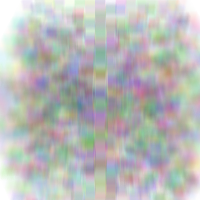
\includegraphics[width=\linewidth]{figs/model0.png}  
\end{subfigure}
\begin{subfigure}{.19\textwidth}
  \centering
  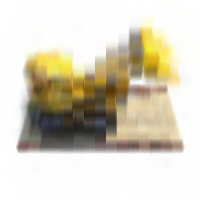
\includegraphics[width=\linewidth]{figs/model1.png}  
\end{subfigure}
\begin{subfigure}{.19\textwidth}
  \centering
  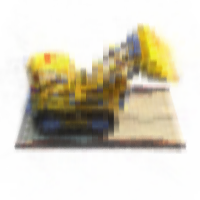
\includegraphics[width=\linewidth]{figs/model3.png}  
\end{subfigure}
\begin{subfigure}{.19\textwidth}
  \centering
  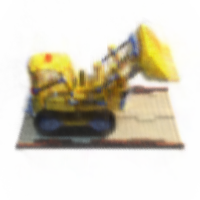
\includegraphics[width=\linewidth]{figs/model15.png}  
\end{subfigure}
\begin{subfigure}{.19\textwidth}
  \centering
  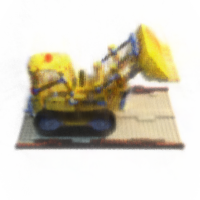
\includegraphics[width=\linewidth]{figs/model32.png}  
\end{subfigure}
     \caption{Our VoxelGrid at epoch {0, 2, 6, 14, 22}. Total computation time: 35 minutes on a single GPU.}
    \label{fig:lego_optim}
\end{figure}


\begin{abstract}
This project report is a study of the article \textbf{Plenoxels: Radiance Fields without Neural Networks} \cite{plenoxels}. Being in the impossibility of using the provided custom CUDA kernel, we have re-implemented the method and a few of the proposed optimizations from scratch. Limiting ourselves to a small 128-sized grid, our implementation achieves a peak-signal-to-noise ratio of $22.10$ dB, not so far from the $23.74$ dB mentioned in the article with a similar setting. We propose two novel extensions: the first one is inspired by \textbf{Space carving} \cite{spacecarving} and allows the generation of clean point clouds from photographs, and the second one relies on a different optimization method and achieves a PSNR of $22.90$ dB. We strongly urge the reader to visit our GitHub repository\footnote{\url{https://github.com/nissmar/Radiance-Fields}} which features animated GIFs, allowing a better viewing of our results (which are on the last page of this report).
\end{abstract}


\section{Introduction}

The most straightforward way to capture 3D objects from the real world is to use special sensors such as the Kinect or more expensive scanning devices. Another approach relies solely on RGB images: by combining photographs taken at several known viewpoints, one is able to render novel views of a scene. A year ago, a method known as \textit{NeRF} (for Neural Radiance Field \cite{nerf}) tackled this challenge by using a deep neural network to simultaneously render shapes and shadings. More recently, a new approach known as \textit{Plenoxels} \cite{plenoxels} showed that directly optimizing a voxel grid allowed better results with faster computations. This project is focused on this paper. In Section \ref{sec:ourimp} we give an overview of our implementation, we review relevant related works in Section \ref{sec:relat}, we present the method and our results in Sections \ref{sec:method} and \ref{sec:results}, and finally, in Section \ref{sec:extent} and \ref{sec:extent2}, we propose our own extension of this method to obtain better point clouds.

\section{Our implementation}\label{sec:ourimp}

\subsection{Given code}


The given code associated to the plenoxels paper requires the compilation of a custom CUDA extension which parallelizes operations. Unfortunately, it requires a CuDNN developer account and quite a bit of C++ experience. In order to avoid losing time on hazardous compilations, we decided to ignore the given code and re-implement everything \textbf{from scratch}, except for the utilities functions \textit{get\_data} and \textit{get\_rays\_np} (30 lines of code) from the original plenoxels repository \footnote{\url{https://github.com/sarafridov/plenoxels}} and the Python file \textit{ply.py}, given in the TP of this course.  

We work on the \textit{nerf\_synthetic} dataset, composed of 8 virtual objects (see Figure \ref{fig:bigresults}).

\subsection{Our goals}


The Plenoxels paper introduces remarkable concepts and the given implementation is no less great: the custom CUDA kernel parrelize across rays, which allow a different number of active voxel for each ray and much faster computations. Reproducing the results was a challenge, and improving the given method (in terms of speed or quality of results) was impossible in the scope of this project.

We thus decided to work with the following constrains: limit ourselves to 128x128x128 size grids (anything bigger is too slow to train with regular tensor multiplications) and measure our results with a reasonable training time (we didn't see the point of day-long optimizations and thus limited ourselves to 30 minutes of training).

\section{Related works}\label{sec:relat}



\subsection{Classical methods}

Before the rise of neural networks, some methods already existed to render novel views from images: one of them is called \textit{Space Carving} \cite{spacecarving}. Starting from a dense grid, the voxels from the surface are removed one by one if they aren't consistent with every photograph. This (quite slow) method successfully captures the 3D shape and texture of the photographed scenes, but is unable to capture the transparent/specular properties of the objects. However, we noticed the rigor of the authors who provide theoretical guarantees, absent from nowadays' optimization methods.

\subsection{NeRF rendering}

The \textit{NeRF} \cite{nerf} approach consists of training a fully-connected network which takes a 5D input $(x,y,z,\theta,\phi)$ composed of a 3D position and a viewing direction, and outputs a 4D tensor $(r, g, b, \sigma)$ composed of an RGB color and an opacity $\sigma$. For each pixel of the rendered image, $N$ points are sampled along a camera ray and their colors and intensities are integrated to obtain a final $RGB$ value. This method achieved state-of-the-art when it was published, as it allowed to reproduce shading and specular effects efficiently. The training time, however, was quite slow (12 hours for a single scene).

\subsection{Concurrent papers and posterior approach}

\textit{DirectVoxGo} \cite{directvoxgo} is similar to Plenoxels: the main differences are that it uses a neural network (and not a custom CUDA implementation). It produces NeRF-comparable results in less than 15 minutes. More recently, a method using multiresolution Hash encoding \cite{instant} was able to reproduce the same results in less than 1 second!

\section{The method}\label{sec:method}

In this section, we'll describe the method of the original paper \cite{plenoxels}, and list the different between their implementation (see Figure \ref{fig:plenoxel}) and ours.



\begin{figure}[!h]
\centering
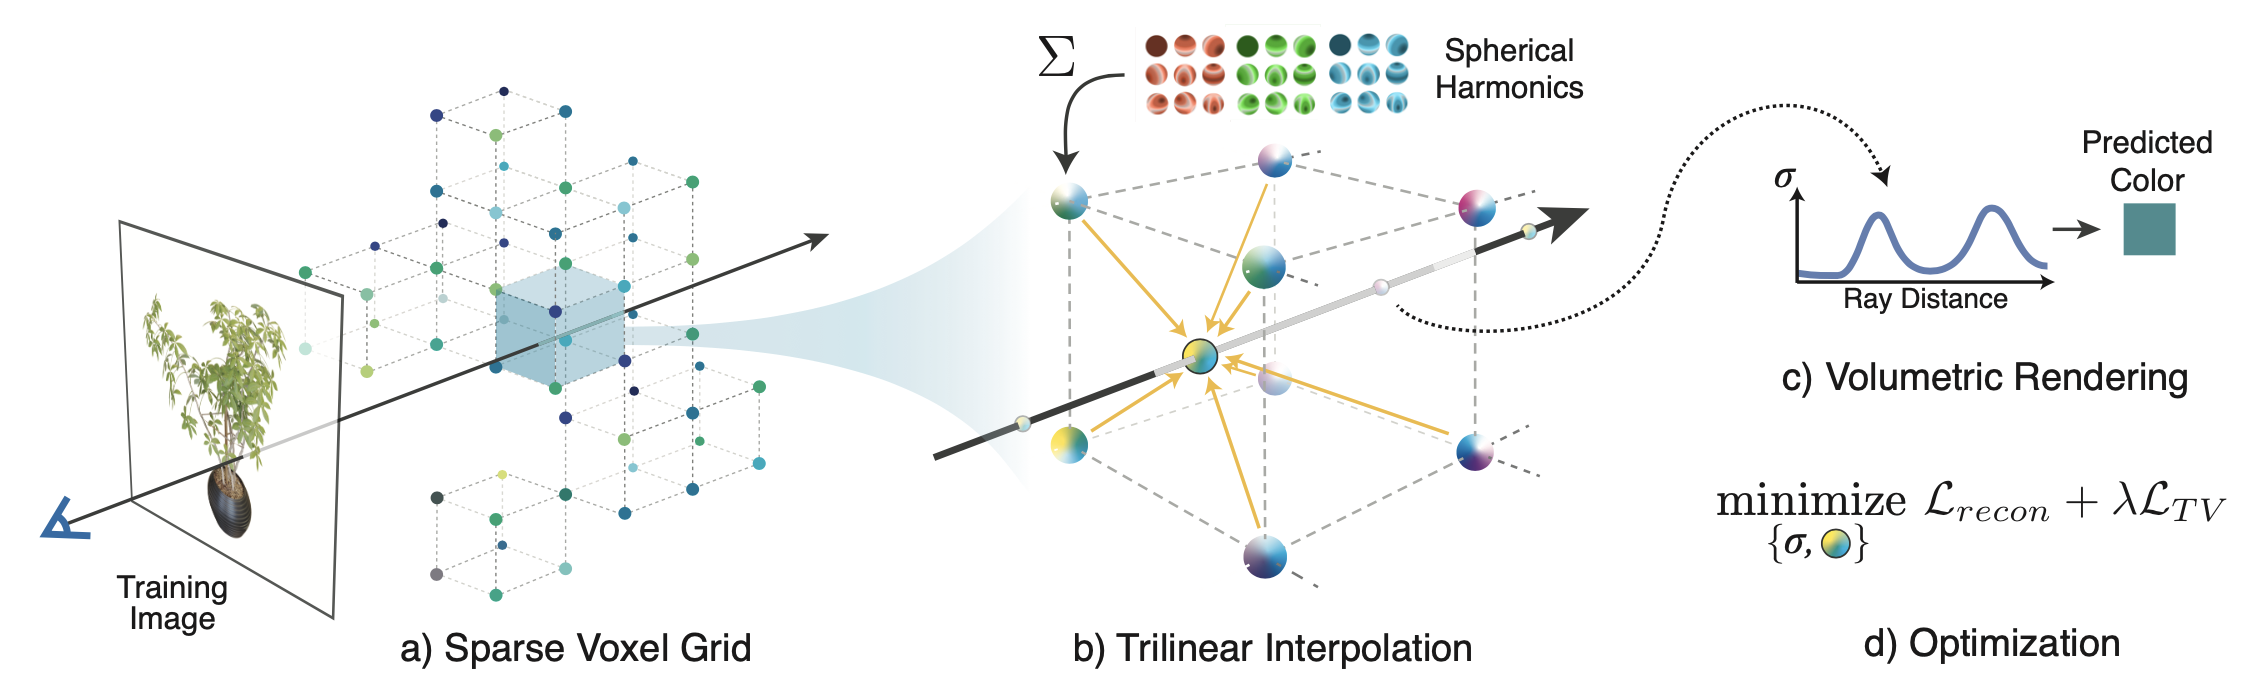
\includegraphics[width=1.\textwidth]{figs/plen_pipeline.png}
\caption{\label{fig:plenoxel} [image source: \cite{plenoxels}] The plenoxels method is composed of four steps : (a) camera rays are extracted from training images and sampled on a sparse voxel grid ; (b) the spherical harmonics of degree 9 and opacities are computed for each sample through trilinear interpolation ; (c) the resulting colors and opacities are summed to obtain a single pixel value for each ray (d) the mean squared error loss with a total variation regularizer is back-propagated to optimize the grid}
\end{figure}



\subsection{Voxel grid and spherical harmonics}

The clever idea of Plenoxels is to optimize a voxel grid directly. Each voxel stores an opacity $\sigma \in \mathbf{R}^+$ along with spherical harmonics coefficients in $[0,1]$. These spherical harmonics allow each voxel to have a different color depending on the viewing direction, which renders specular effects and reflections.

\begin{figure}[!h]
 \centering
\begin{subfigure}{.1\textwidth}
  \centering
  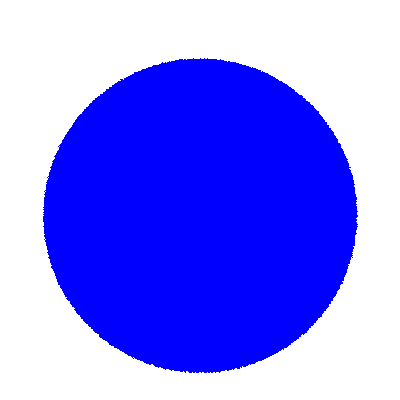
\includegraphics[width=\linewidth]{figs/spherical_harmonics/harmonics_0.png}  
\end{subfigure}
\begin{subfigure}{.1\textwidth}
  \centering
  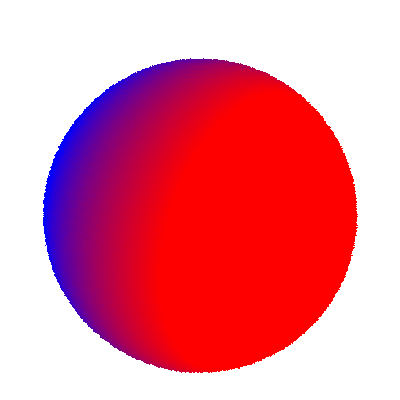
\includegraphics[width=\linewidth]{figs/spherical_harmonics/harmonics_1.png}  
\end{subfigure}
\begin{subfigure}{.1\textwidth}
  \centering
  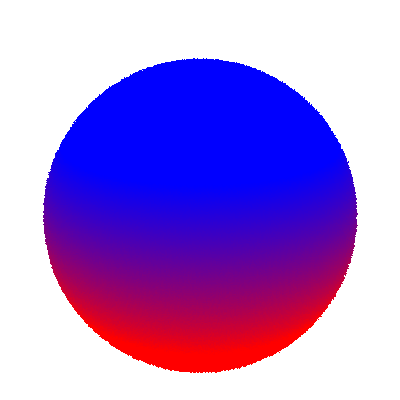
\includegraphics[width=\linewidth]{figs/spherical_harmonics/harmonics_2.png}  
\end{subfigure}
\begin{subfigure}{.1\textwidth}
  \centering
  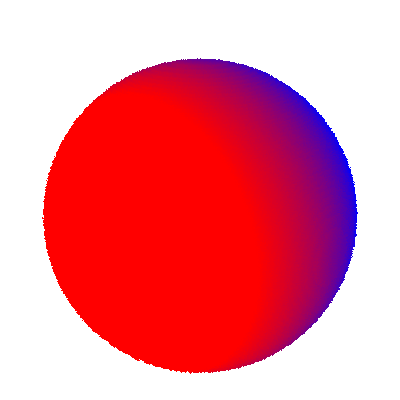
\includegraphics[width=\linewidth]{figs/spherical_harmonics/harmonics_3.png}  
\end{subfigure}
\begin{subfigure}{.1\textwidth}
  \centering
  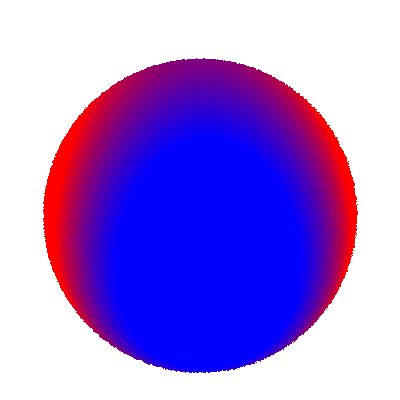
\includegraphics[width=\linewidth]{figs/spherical_harmonics/harmonics_4.png}  
\end{subfigure}
\begin{subfigure}{.1\textwidth}
  \centering
  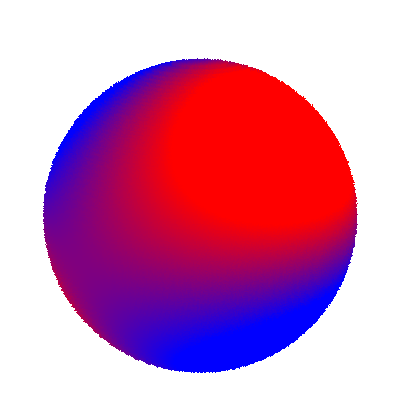
\includegraphics[width=\linewidth]{figs/spherical_harmonics/harmonics_5.png}  
\end{subfigure}
\begin{subfigure}{.1\textwidth}
  \centering
  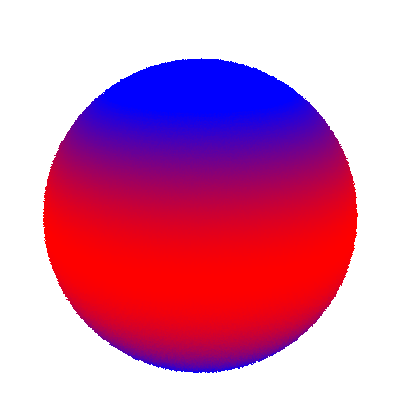
\includegraphics[width=\linewidth]{figs/spherical_harmonics/harmonics_6.png}  
\end{subfigure}
\begin{subfigure}{.1\textwidth}
  \centering
  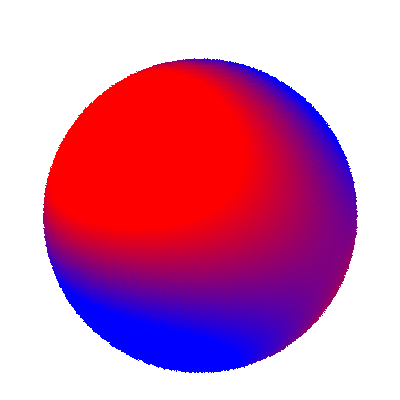
\includegraphics[width=\linewidth]{figs/spherical_harmonics/harmonics_7.png}  
\end{subfigure}
\begin{subfigure}{.1\textwidth}
  \centering
  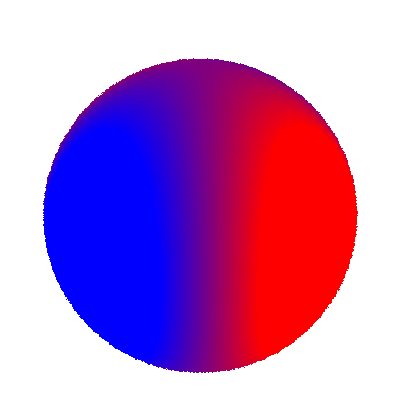
\includegraphics[width=\linewidth]{figs/spherical_harmonics/harmonics_8.png}  
\end{subfigure}
     \caption{Spherical harmonics of order 1 to 9}
    \label{fig:sph_harm}
\end{figure}


The original paper uses a sparse voxel grid optimized with the custom CUDA implementation. Ours is a dense voxel grid which which justifies the lower definition (128x128x128 vs 512x512x512) and the longer computation time. We experimented with spherical harmonics of degree 1 (each voxel has a single color), and 9, but the latter was to slow to trained. The Plenoxels paper doesn't give the detail of which harmonics they're using, and even though the ones on Figure \ref{fig:plenoxel} seem to have values in [0,1], we believe they use spherical harmonics with values in [-1,1] (Figure \ref{fig:sph_harm}). These are the ones we use in our extension (Section \ref{sec:extent2}).

\subsection{Color estimation from camera rays}

Once this grid is initialized at random, we optimize its voxels based on images taken from known viewpoints. Each pixel $p_x$ of the training images corresponds to a certain camera ray $r(p_x) \in (\mathbf{R}^3, \mathbf{R}^3)$ composed of an origin and a direction. We sample this ray with $N=200$ points, compute the points colors and opacities via nearest neighbour interpolation (we implemented trilinear interpolation like in the paper but it was 8 times slower) and sum the sampled points to obtain the estimated RGB color $\hat{c}(r(p_x))$:
\[\hat{c}(r(p_x)) = \sum_{0\leq i<N} T_i (1 - \exp(-\sigma_i \delta_i)) c_i\] 

Where $ T_i = \exp(- \sum_{0\leq j<i} \sigma_j \delta_j)$ represents how much light is transmitted to sample $i$ and $\delta_i$ represents the distance between samples.\\ 

At first, we were quite puzzled at by this formula, so we considered the following example: an object of constant color $c$ and opacity $\sigma$ sampled by $N$ points. The distance between points is thus $D/N$, where $D$ is a constant. The resulting color of a ray through this material is:
\[ \sum_{1 \leq i \leq N} \exp(- (i-1)\frac{ \sigma D}{N})(1 - \exp(-  \frac{ \sigma D}{N}))c = c (1 - exp(- \sigma D))\]

In this simple case, the color is indeed independent from the number of samples. When $N \rightarrow + \infty$, the render will converge (note that it assumes however constant values of color and opacity between samples). In our experiment, we decided to take $N$ sufficiently large so that the distance between samples isn't too big compared to the voxel size.


\subsection{Optimization}
The loss is the Mean Squared Error: $L = \sum_{p_x} \|p_x -\hat{c}(r(p_x)) \|^2 + \lambda_{TV}  L_{TV}$, and back-propagate through the grid. At each training step, we sample 5000 random rays and compute the total variation over the whole grid. We used an SGD optimizer to do the gradient descent with a learning rate of 1000, and $\lambda_{TV} = 10^{-4}$. 

\section{Results and experiments}\label{sec:results}

\subsection{Visual interpretation}

%\begin{figure}[!h]
% \centering
%
%\begin{subfigure}{.24\textwidth}
%  \centering
%  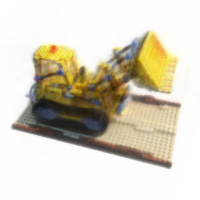
\includegraphics[width=\linewidth]{figs/results/lego.png}  
%\end{subfigure}
%\begin{subfigure}{.24\textwidth}
%  \centering
%  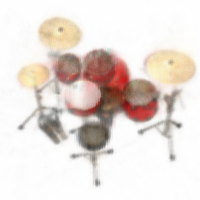
\includegraphics[width=\linewidth]{figs/results/drums.png}  
%\end{subfigure}
%\begin{subfigure}{.24\textwidth}
%  \centering
%  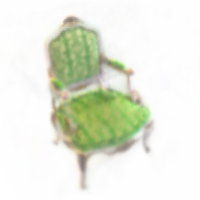
\includegraphics[width=\linewidth]{figs/results/chair.png}  
%\end{subfigure}
%\begin{subfigure}{.24\textwidth}
%  \centering
%  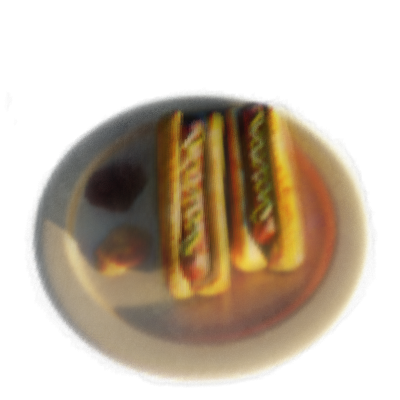
\includegraphics[width=\linewidth]{figs/results/hotdog.png}  
%\end{subfigure}
%\begin{subfigure}{.24\textwidth}
%  \centering
%  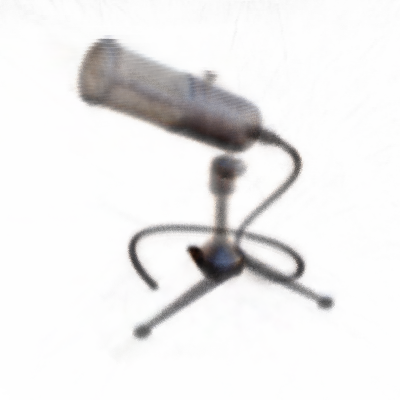
\includegraphics[width=\linewidth]{figs/results/mic.png}  
%\end{subfigure}
%\begin{subfigure}{.24\textwidth}
%  \centering
%  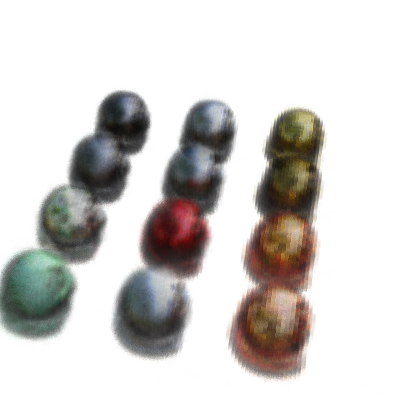
\includegraphics[width=\linewidth]{figs/results/materials.png}  
%\end{subfigure}
%\begin{subfigure}{.24\textwidth}
%  \centering
%  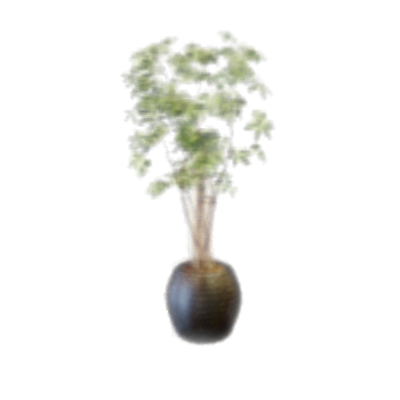
\includegraphics[width=\linewidth]{figs/results/ficus.png}  
%\end{subfigure}
%\begin{subfigure}{.24\textwidth}
%  \centering
%  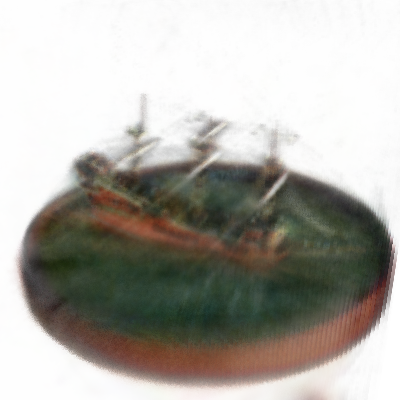
\includegraphics[width=\linewidth]{figs/results/ship.png}  
%\end{subfigure}
%     \caption{Our models evaluated on novel viewpoints (see our GitHub repository for animated GIFs)}
%    \label{fig:results}
%\end{figure}

The result of our Plenoxels implementation is visible in Figure \ref{fig:bigresults} (at the end of this report, in the column \textit{Voxel Grid}). Considering the fact that we couldn't use a custom CUDA kernel, we are quite satisfied with our results. They are visually plausible, even though at slight blur is noticeable: as we use spherical harmonics of degree 1, specular effects aren't rendered, and we believe this blur minimizes the color variations. Visually, the ship is the least realistic: because of its small details, a grid of size 128x128x128 isn't sufficient to represent it. We were impressed with the mic and its semi-transparent wire mesh.

\subsection{PSNR comparison}

The PSNR (for peak signal to noise ratio), defined as $PSNR = 10\log_{10}(1/MSE)$, is an image metric often used in image restoration. In this context, novel test views are used to compare the rendered model and the real image. In the original paper, a score of $23.73$ dB is reached with a 128x128x128 grid and nearest neighbor interpolation. We obtain a score of $22.10$ dB (see Table \ref{tab:psnr}). We are quite satisfied with this result, considering the fact that we only use spherical harmonics of order 1. We verified a statement of the paper: TV regularization doesn't bring better results in those synthetic scenes. Surprisingly, the ficus has a higher PSNR than the chair, although the latter looks much better: this metric compares pixel values, and not shape consistency. 

\subsection{Adaptative grid size for faster optimization}


\begin{figure}[!h]
\centering
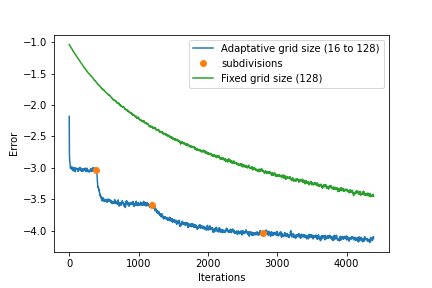
\includegraphics[width=0.5\textwidth]{figs/training_mic.png}
\caption{\label{fig:subd} Evolution of the error curve on the microphone model}
\end{figure}

In the paper, they subdivide the voxel grid via tri-linear interpolation to boost the training phase. We tested and implemented this method which greatly accelerated our optimization (Figures \ref{fig:lego_optim} and \ref{fig:subd}). We use grids of size ${16, 32, 64, 128}$, on respectively ${2, 4, 8, 8}$ epochs with a learning rate of ${1000, 1000, 500, 500}$. We use trilinear interpolation on colors and opacities to subdivide the grid.



\subsection{Using plenoxels to generate point clouds: CloudCompare pipeline}


\begin{figure}[!h]
 \centering
\begin{subfigure}{.24\textwidth}
  \centering
  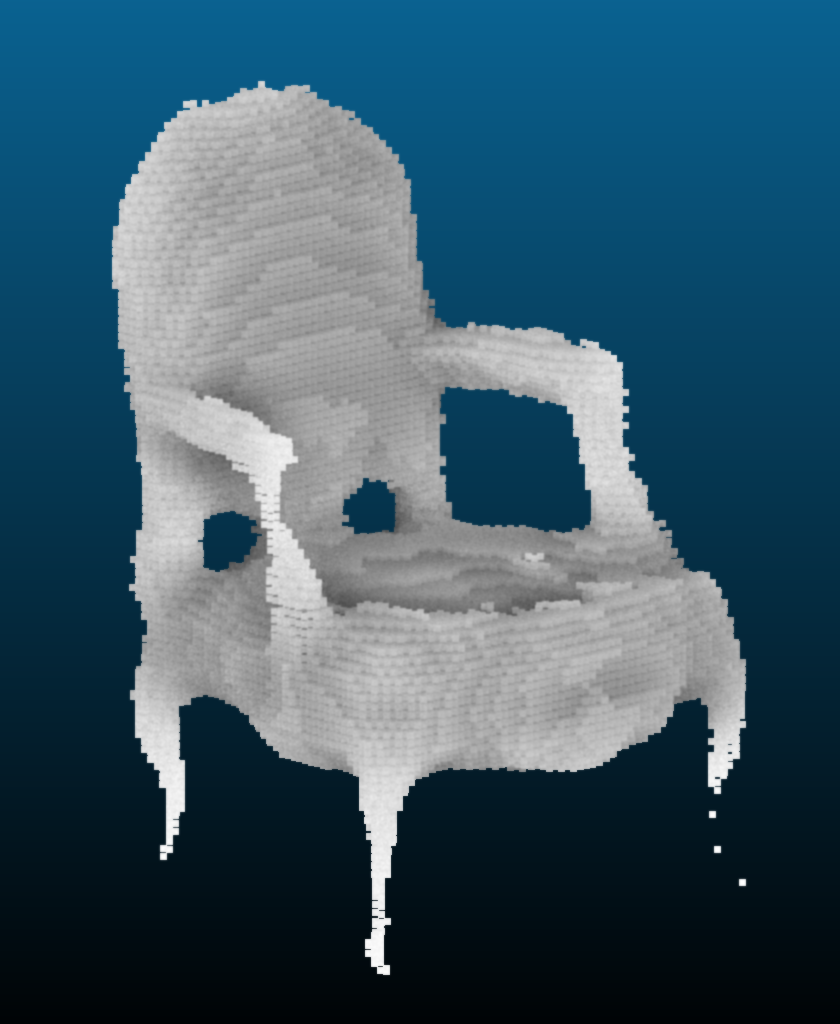
\includegraphics[width=\linewidth]{figs/pc/chair.png}  
\end{subfigure}
\begin{subfigure}{.24\textwidth}
  \centering
  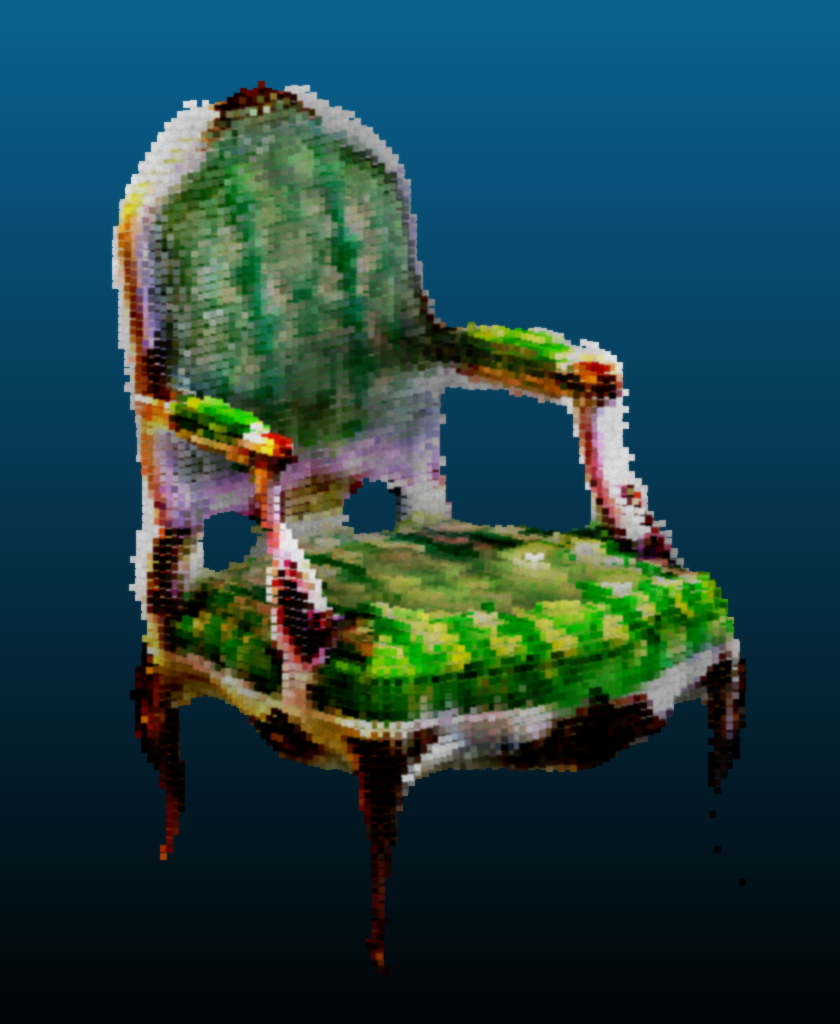
\includegraphics[width=\linewidth]{figs/pc/chairc.png}  
\end{subfigure}
\begin{subfigure}{.24\textwidth}
  \centering
  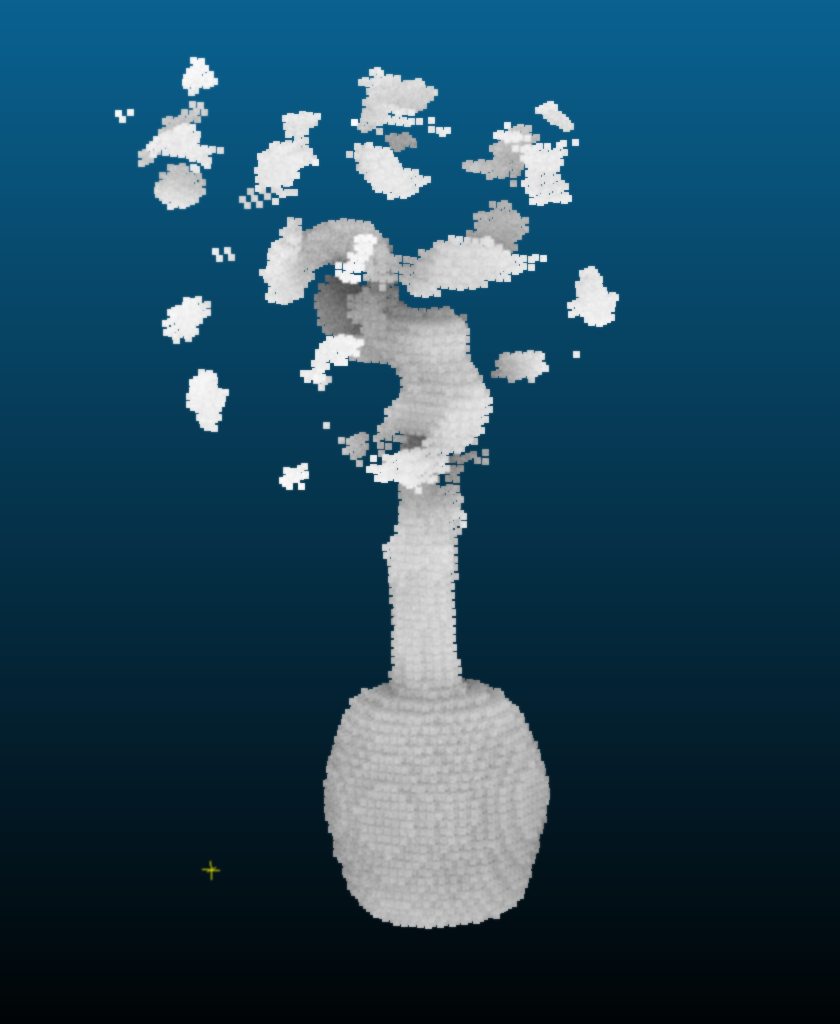
\includegraphics[width=\linewidth]{figs/pc/ficus.png}  
\end{subfigure}
\begin{subfigure}{.24\textwidth}
  \centering
  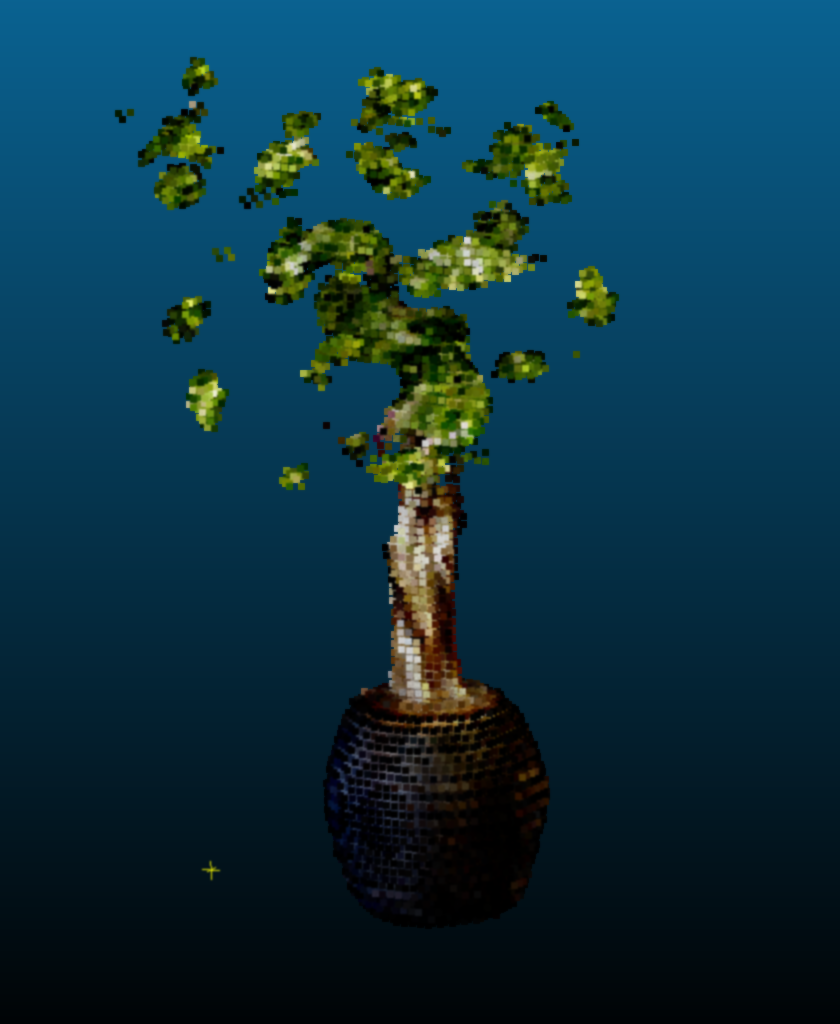
\includegraphics[width=\linewidth]{figs/pc/ficusc.png}  
\end{subfigure}
     \caption{Chair and ficus models loaded in CloudCompare}
    \label{fig:cc}
\end{figure}

A point cloud can be seen as a voxel grid with discrete (0 or 1) opacities. We implemented a \textit{.ply} export of our voxel grids, storing the RGB colors and the opacity as a scalar field. 

We found that applying the following transformations helped clean the result in CloudCompare:

\begin{itemize}
\item \textbf{Edit $>$ Scalar fields $>$ Filter by value} (Range $2.0; +\infty$) to remove the transparent voxels
\item \textbf{Tools $>$ Clean $>$ Noise filter} (Radius $0.01$) to clean the point cloud
\item \textbf{Tools $>$ Clean $>$ S.O.R. filter} (Radius $0.2$) to remove the outliers.
\end{itemize}


The optimal parameters may vary for each model (little less value filter for the lego model, little more noise filter for the hotdog model..). Although the colors are transferred efficiently, the shape is imprecise as the opacities aren't binary: some white clouds remain (for instance on the arm of the chair), and filtering them may lead to the destruction of tiny details (such as the leaves of the ficus). We imagined and implemented a new method to obtain better quality results: this is what we'll see now.

\section{First extension: deterministic voxel grid optimization}\label{sec:extent}

\subsection{The idea}

Since the \textit{nerf\_synthetic} photographs have a transparent background, some of the rays shouldn't hit any voxels (we call them \textit{transparent rays}). Inspired by space carving \cite{spacecarving}, we implemented an algorithm to filter them. First we set every opacity to a constant $\sigma$ (we set it fairly high to have almost opaque voxels). Then we remove the voxels which are on the path of transparent rays. Once the voxel grid has been carved, the colors are added: instead of optimizing the complicated loss $L = \sum_{p_x} \|p_x -\hat{c}(r(p_x)) \|^2$, we average the colors of the corresponding pixels, with weights proportional to the opacity in each visit. We found that using $\tilde{c_v} = \frac{ \sum_{r \in R_v} T_{i,r}  (1 - \exp(-\sigma \delta_i)) p_r }{ \sum_{r \in R_v} T_{i,r}  (1 - \exp(-\sigma \delta_i))  }$ where $R_v$ is the set of all rays passing through voxel $v$, yielded the best results. This method is lightning fast, as it requires only 2 passes through the dataset to obtain the final shape: a 128x128x128 grid can be obtained in 1 minute (the relevant python file is \textit{main\_carve.py}).

\subsection{Results}

\begin{figure}[!h]
 \centering
\begin{subfigure}{.24\textwidth}
  \centering
  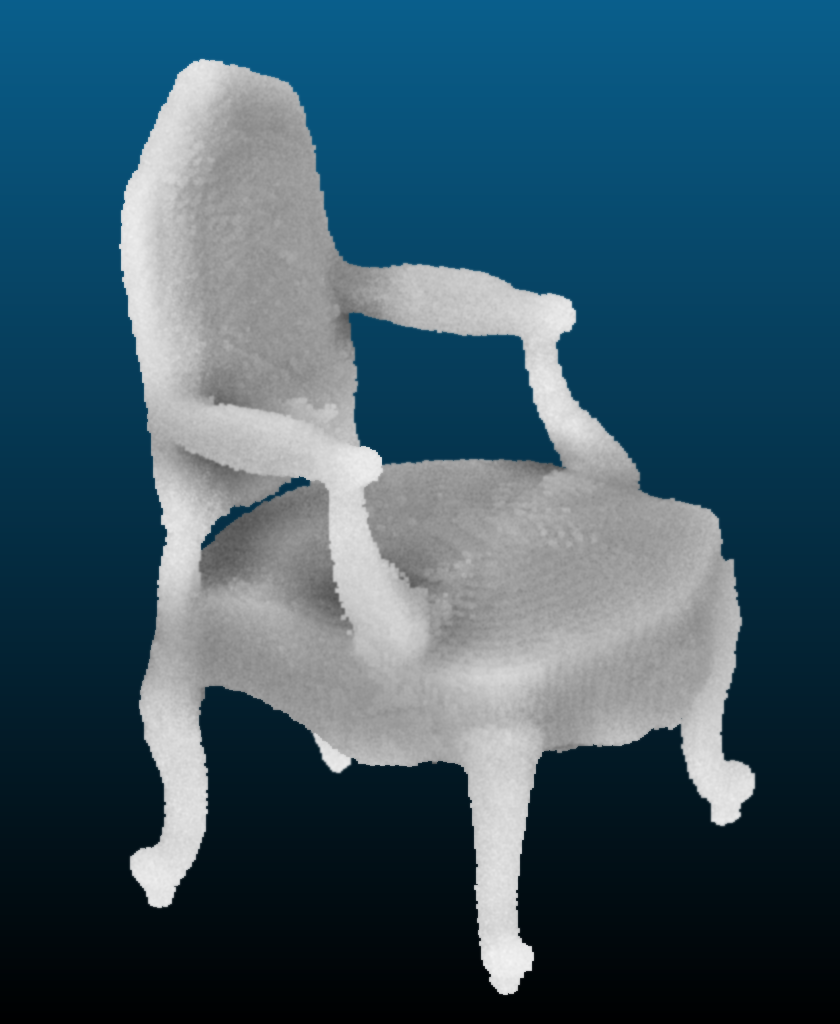
\includegraphics[width=\linewidth]{figs/carve/chair.png}  
\end{subfigure}
\begin{subfigure}{.24\textwidth}
  \centering
  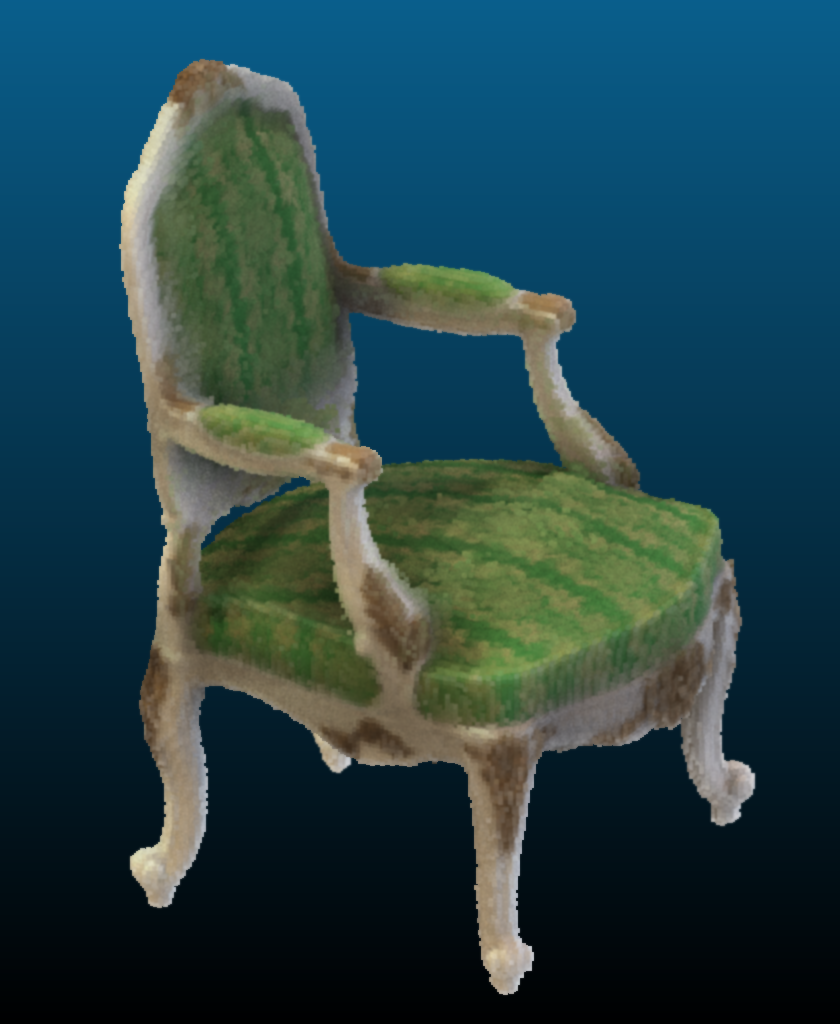
\includegraphics[width=\linewidth]{figs/carve/chairc.png}  
\end{subfigure}
\begin{subfigure}{.24\textwidth}
  \centering
  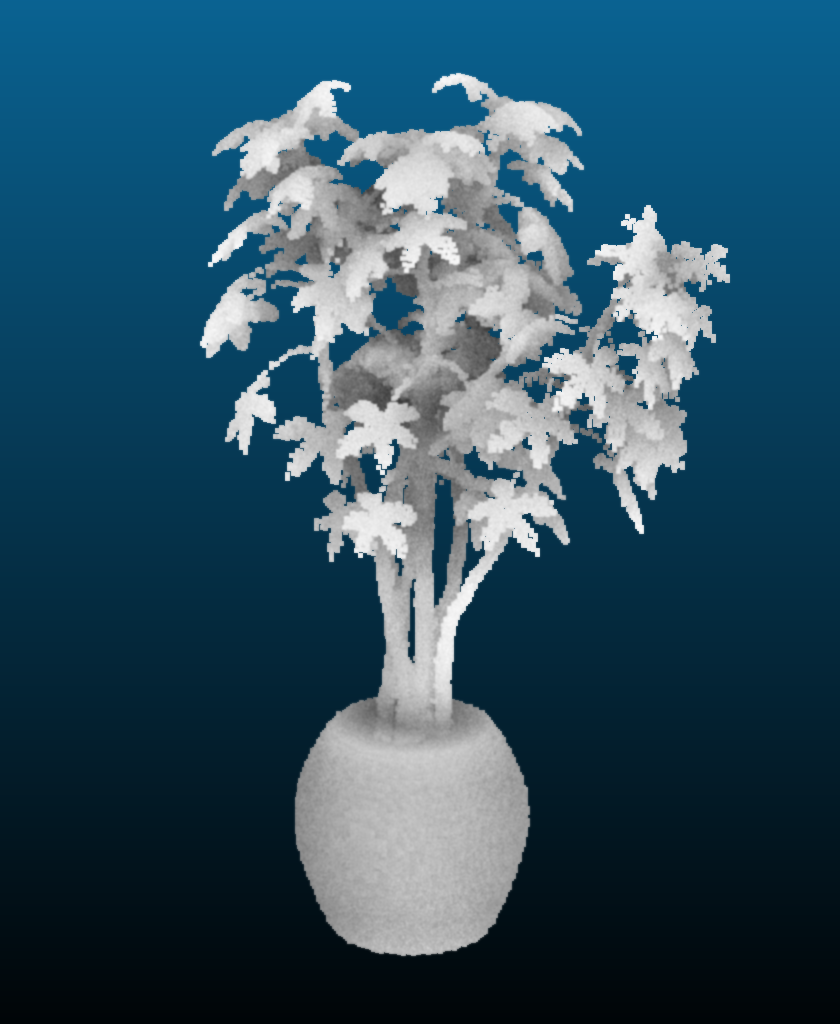
\includegraphics[width=\linewidth]{figs/carve/ficus.png}  
\end{subfigure}
\begin{subfigure}{.24\textwidth}
  \centering
  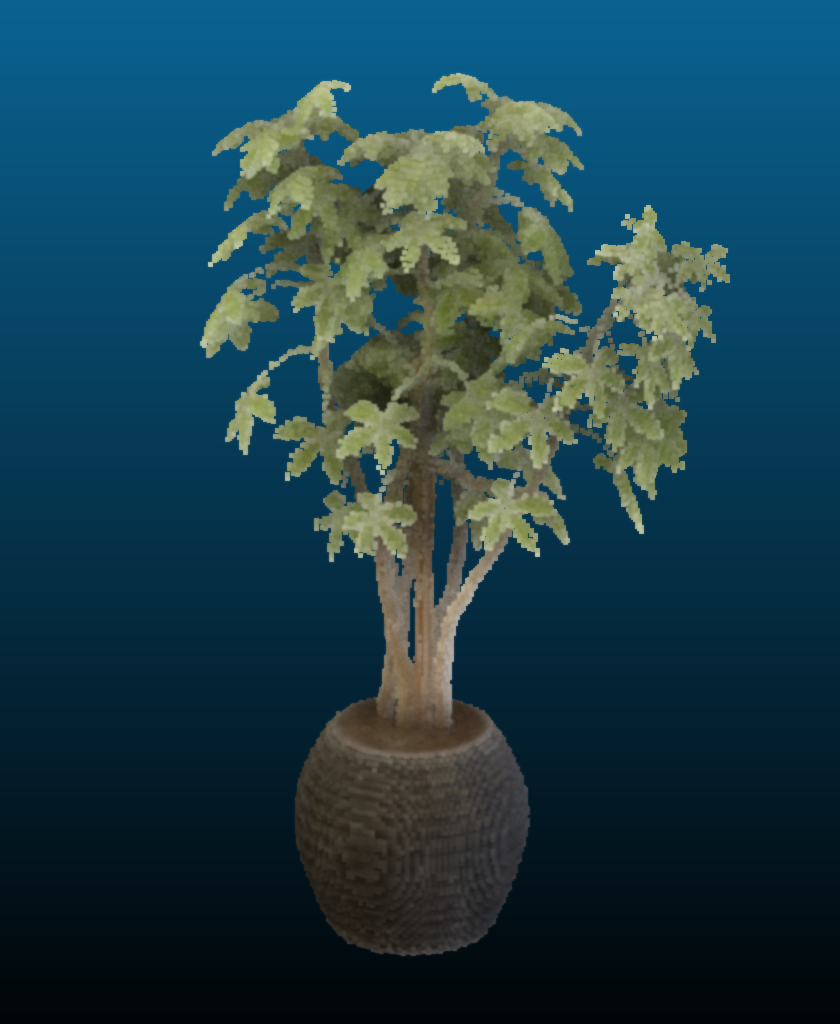
\includegraphics[width=\linewidth]{figs/carve/ficusc.png}  
\end{subfigure}
     \caption{Chair and ficus models obtained with our method}
    \label{fig:cc2}
\end{figure}

The obtained pointclouds are much cleaner and usable (Figure \ref{fig:cc2}), although some artifacts may appear (for instance on the wheels of the lego model, Figure \ref{fig:ourccdetail}). Since the color of every voxel $\tilde{c_v}$ is estimated, the whole material is colored (Figure \ref{fig:legod2}), which we believe is more robust. In the concave parts of the model, the voxels aren't removed, which leads to inaccuracies (Figure \ref{fig:legod3}). Even if the user doesn't need a point cloud, this approach shows clearly which voxels are visible in the training set: we believe it can be useful to create new nerf-compatible scenes. Working with transparent backgrounds shouldn't be an issue: even for real objects they can be easily obtained with segmentation tools. 


\begin{figure}[!h]
 \centering
\begin{subfigure}{.32\textwidth}
  \centering
  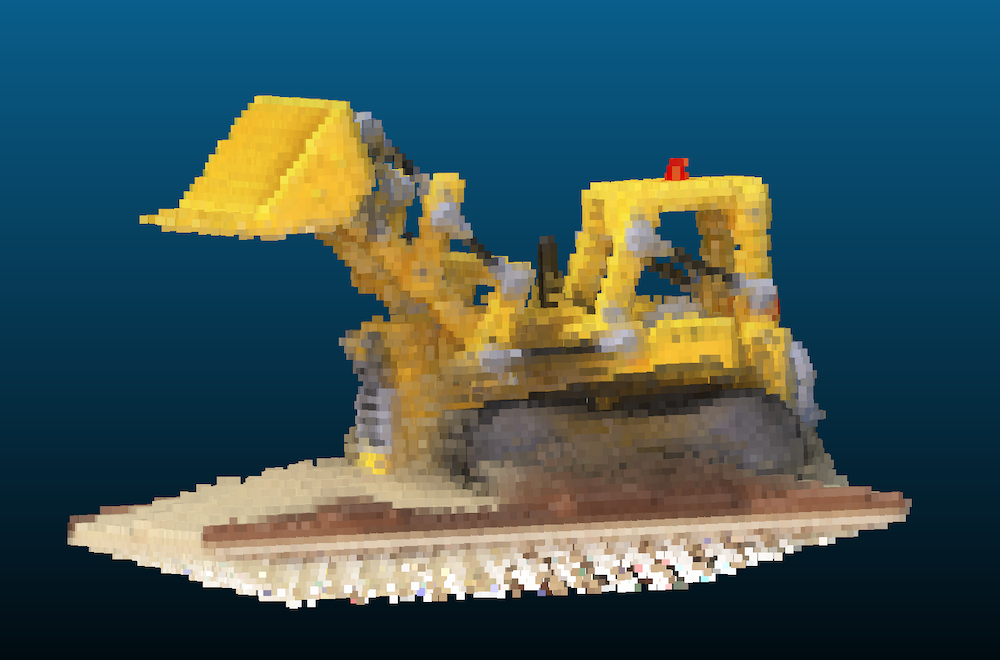
\includegraphics[width=\linewidth]{figs/carve/legod1.png}   \caption{\label{fig:legod1} The full model}
\end{subfigure}
\begin{subfigure}{.32\textwidth}
  \centering
  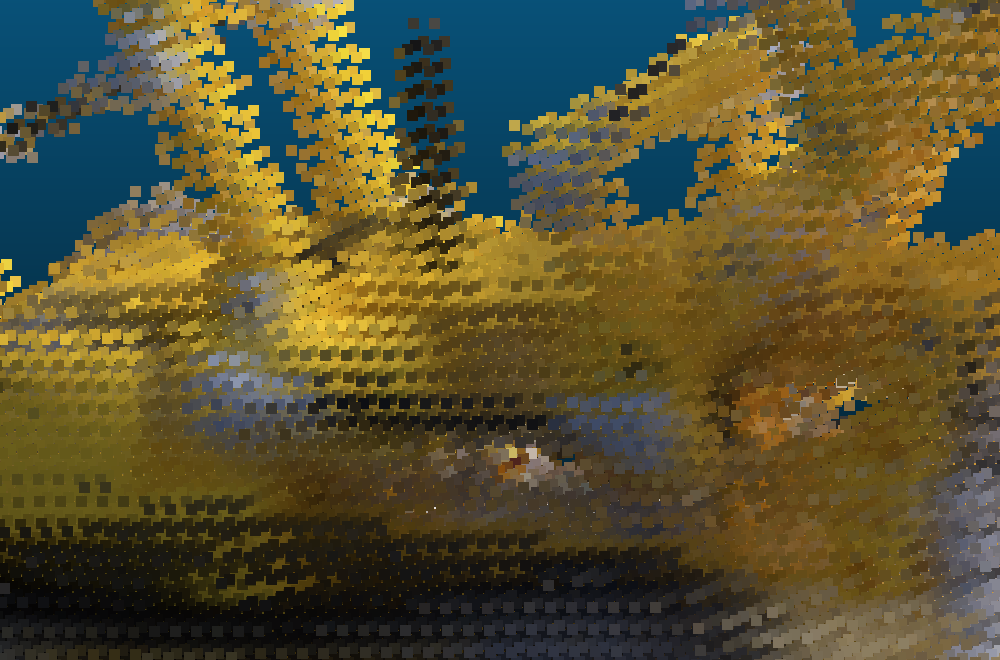
\includegraphics[width=\linewidth]{figs/carve/legod2.png}   \caption{\label{fig:legod2} Each voxel is colored }
\end{subfigure}
\begin{subfigure}{.32\textwidth}
  \centering
  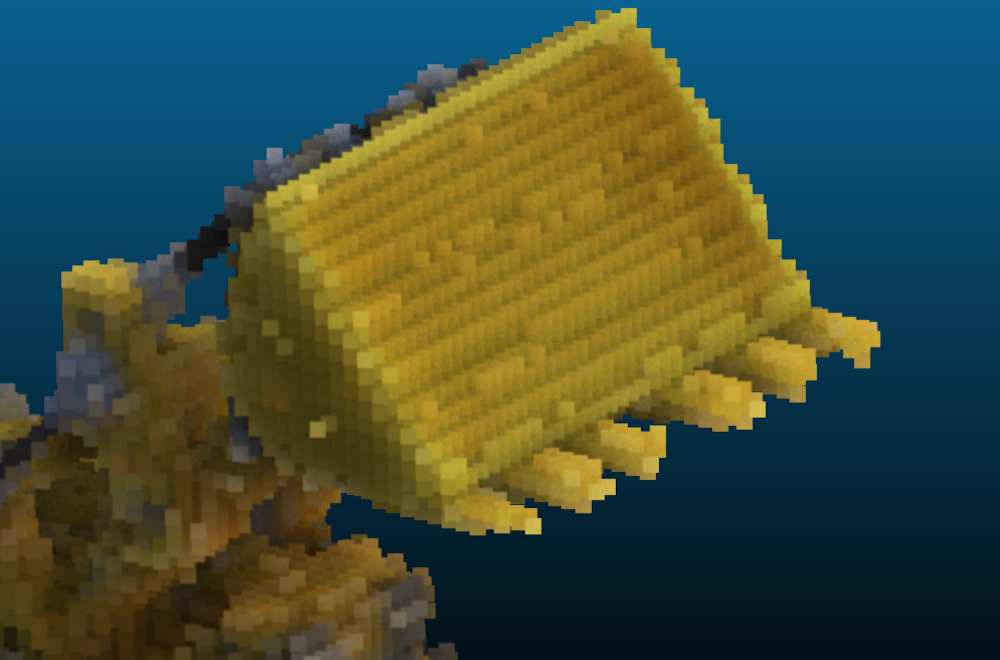
\includegraphics[width=\linewidth]{figs/carve/legod3.png}   \caption{\label{fig:legod3}  Concave shaped are filled}
\end{subfigure}
   \caption{Details of our the lego model}
    \label{fig:ourccdetail}
\end{figure}

The efficiency of that method made using spherical harmonics possible: this is what we will present in the next section.

\section{Second extension: quick spherical harmonics}\label{sec:extent2}

\subsection{The idea}
The second algorithm extends the one described in the previous section: the first steps are identical, with the exception of setting the first spherical harmonics instead of the whole color of the pixel (note that in this case each voxel stores 9x3 coefficients). Since we have set the opacities to a high value, we can consider that each voxel is either transparent or visible. The pseudo-loss is $L = \sum_{v} \sum_{p_x hitting v} \|p_x - S_{r(p_x)}^T c_v\|^2$. For each voxel and each ray, the gradient can be computed, and is equal to $ -2 S_{r(p_x)} (p_x - S_{r(p_x)}^T c_v)^T$. This fastens up computations, and we optimize our grid directly with SGD and a decaying learning rate going from 0.9 to 0.1.

\subsection{Results}

The results can be seen in Figure \ref{fig:bigresults}. The results are a massive improvement from the previous two methods as the objects are more vivid and better defined. The specular properties of the chair's ornaments, the bronze-like material, the mic and its handle are rendered. There is one phenomenon we didn't expect: the spherical harmonics "trick" the viewer and make some objects disappear depending on the angle: it's the case for the lego's wheel, the side of the ship's box...  These improvements are confirmed by the PSNR (see Table \ref{tab:psnr}), as they're the highest of all our tests. 

\newpage

\section{Conclusion}

Re-implementing Plenoxels from scratch was definitely a challenge: their using of a non-standard CUDA kernel should have warned us of the underlying complexity. As the algorithm relies on an optimization, mistakes often go unnoticed and the debugging is particularly hard. Nevertheless, we are quite satisfied with the results our substantial amount of code (600 lines for the file \textit{VoxelGrid.py} alone)  provides, close in PSNR to the results obtained in the article with a 128 grid and nearest-neighbor interpolation.

We expected that their method would easily translate to point cloud generation, but it isn't the case: as shown in the last section, we believe it's because the differentiable rendering only creates a mere \textit{illusion} of shape. Our extensions mitigate this problem, although they aren't able to carve out concavities in the rendered objects.

A possible extension to our work would be to merge the two approaches, and start the plenoxels optimization from an already carved grid.


\bibliographystyle{alpha}
\bibliography{sample}

\begin{table}[!h]
\centering
\begin{tabular}{|l||c|c|c|r|}
\hline
Dataset & VoxelGrid + TV & VoxelGrid & VoxelGridCarve & VoxelGridSphericalCarve \\\hline
Drums & 20.12 dB & 20.12 dB  & 19.32 dB & 19.72 dB\\
Chair & 23.69 dB & 23.70 dB & 24.22 dB & 26.94 dB \\ 
Ship & 20.65  dB & 20.66 dB & 20.25 dB &  21.91 dB\\
Ficus & 23.86 dB & 23.85 dB & 21.90 dB & 21.66 dB\\
HotDog &  23.79 dB &  23.75 dB & 23.45 dB & 25.99 dB  \\
Materials &  20.98 dB &  20.99 dB & 19.715 dB & 22.41 dB \\
Lego &   21.43 dB &  21.42 dB  & 20.72 dB & 22.94 dB \\
Mic &  22.32 dB & 22.29 dB  & 20.63 dB & 21.62 dB\\
\hline 
Mean & 22.10 ± 1.41  dB & 22.10 ± 1.41 dB & 21.28 ± 1.65 dB & 22.90 ± 2.24 dB \\
\hline\hline
Training Time & 35 minutes & 35 minutes & 1 minute & 4 minutes \\
\hline 
\end{tabular}
\caption{\label{tab:psnr}PSNR on different training methods.}
\end{table}

\newpage

\newcommand{\animage}[1][example-image]{\adjustbox{valign=m,vspace=0pt}{\includegraphics[width=.18\linewidth]{#1}}}

\begin{figure}
\centering
\begin{tabular}{cccc}
Ground truth & VoxelGrid & VoxelGridCarve & VoxelGridSphericalCarve \\
       
       
\animage[figs/comp/chair.png]  & \animage[figs/comp/vg_chair.png] & \animage[figs/comp/vgc_chair.png] & \animage[figs/comp/vgcs_chair.png] \\

\animage[figs/comp/materials.png]  & \animage[figs/comp/vg_materials.png] & \animage[figs/comp/vgc_materials.png] & \animage[figs/comp/vgcs_materials.png] \\

\animage[figs/comp/mic.png]  & \animage[figs/comp/vg_mic.png] & \animage[figs/comp/vgc_mic.png] & \animage[figs/comp/vgcs_mic.png] \\


\animage[figs/comp/lego.png]  & \animage[figs/comp/vg_lego.png] & \animage[figs/comp/vgc_lego.png] & \animage[figs/comp/vgcs_lego.png] \\

\animage[figs/comp/drums.png]  & \animage[figs/comp/vg_drums.png] & \animage[figs/comp/vgc_drums.png] & \animage[figs/comp/vgcs_drums.png] \\

\animage[figs/comp/ficus.png]  & \animage[figs/comp/vg_ficus.png] & \animage[figs/comp/vgc_ficus.png] & \animage[figs/comp/vgcs_ficus.png] \\


\animage[figs/comp/hotdog.png]  & \animage[figs/comp/vg_hotdog.png] & \animage[figs/comp/vgc_hotdog.png] & \animage[figs/comp/vgcs_hotdog.png] \\


\animage[figs/comp/ship.png]  & \animage[figs/comp/vg_ship.png] & \animage[figs/comp/vgc_ship.png] & \animage[figs/comp/vgcs_ship.png] \\
\end{tabular}
\caption{\label{fig:bigresults} Our models evaluated on novel test views}
\end{figure}



\end{document}
